\pagestyle{fancy}
\renewcommand{\theUnit}{1}
\ifthenelse{\isundefined{\UnitPageNumbers}}{}{\setcounter{page}{1}}
\rhead{Chapter \theUnit: Data and Case Studies}
\lhead{Math 3382: Statistical Theory}
%\lhead{
\includegraphics[width=1.25cm]{CUDenver-Logo.png}}
\rfoot{\mypage}
\cfoot{
\includegraphics[width=2.25cm]{CUDenver-Logo-coverpage.png}}
\lfoot{Adam Spiegler}
\fancypagestyle{firstfooter}{\footskip = 50pt}
\renewcommand{\footrulewidth}{.4pt}
%%%%%%%%%%%%%%%%%%%%%%%%%%%
\vspace*{-20pt} \thispagestyle{firstfooter}


%\begin{tasks}[counter-format = {(tsk[a])},label-offset = {0.8em},label-format = {\color{black}\bfseries}](2)

\pagebegin{Introduction to Statistical Inference}

%\textbf{\textcolor{blue}{Probability}} is the branch of mathematics concerning numerical descriptions of how likely an event is to occur.
%\bi
%\ii Suppose 1\% of the lithium batteries produced by a certain manufacturer are known to be defective. How likely is it that a shipment of 20 batteries has no defective batteries?
%\ei
%\bi
%\ii What proportion of all lithium batteries produced by a manufacturer are defective? You pick a sample of 500 batteries from this manufacturer, and find that $1.5$\% of the batteries in the sample are defective. What proportion of all batteries produced by this manufacturer are defective?
%\ei

\bbox
\textbf{\textcolor{blue}{Statistics}} is the study of collection, organization, analysis, interpretation, and presentation of data.
\ebox

To get things started, consider the following example. The General Social Survey (GSS) is a major survey that tracks demographics, characteristics, views, and opinions.


\begin{center}
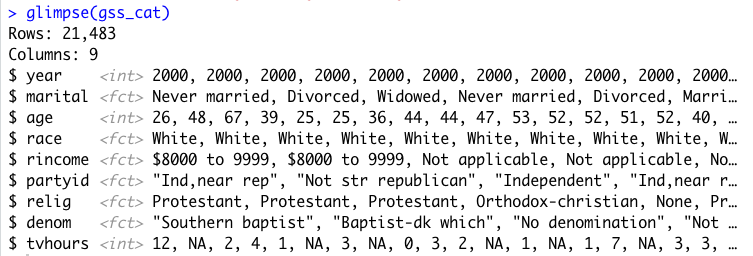
\includegraphics[width=6in]{01/fig-glimpse.png}
\end{center}

\bb
\ii What do you notice about the dataset gss\_cat? How would you summarize what information is contained in this dataset? \vfill
\ii What additional information would be nice to know about this dataset? \vfill
\ee


\clearpage

\pagebegin{The Language of Data}

\bbox
\bi
\ii A \textbf{\colorb{variable}} is a characteristic you can measure. If the property:
\bi
\ii Is measured or counted by a number, it is a \textbf{\colorb{quantitative or numerical}} variable.
\ii Places individuals/objects into groups or categories, it is a \textbf{\colorb{qualitative or categorical}} variable.
\ei
\ii An \textbf{\colorb{observation}} is a set of measurements made under similar conditions. An observation will contain several values, each associated with a different variable.
\ii \textbf{\colorb{Tabular data}} is a set of values, each associated with a variable and an observation.
\bi
\ii Tabular data is \textbf{\colorb{tidy}} if each row corresponds to a different observation and column corresponds to a different variable.
\ei
\ei
\ebox

\begin{center}
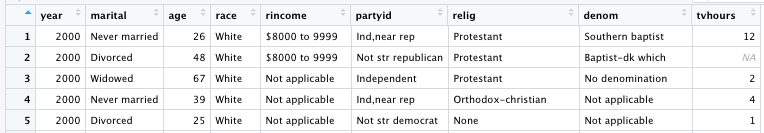
\includegraphics[width=7in]{01/fig-view.png}
\end{center}

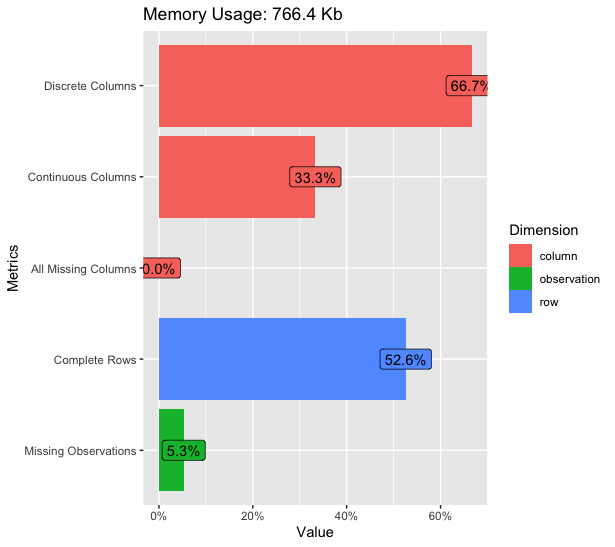
\includegraphics[width=4in]{01/fig-plot-intro.png} \ \ \ \ \ \ 
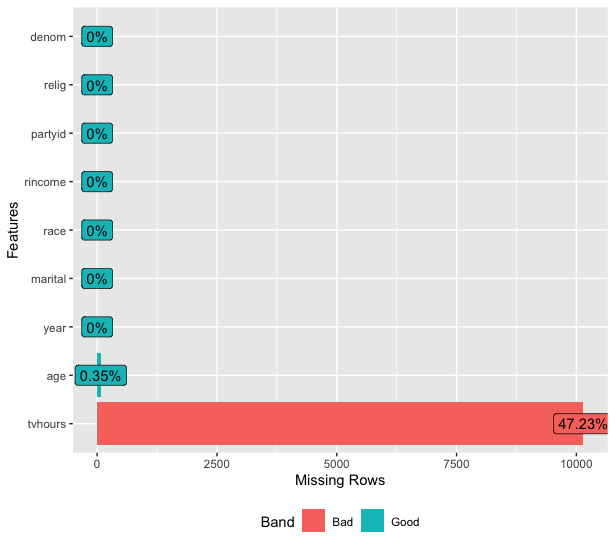
\includegraphics[width=3in]{01/fig-plot-missing.png}

\clearpage

\pagebegin{Presentation of Data}

That type of analysis we can do depending on whether:
\bi
\ii We are investigating a single variable, or looking for correlation between multiple variables.
\ii The variable(s) are numerical and/or categorical.
\ii The data satisfies certain assumptions.
\ei

The distribution of values for a numerical variable is often displayed using a \textbf{\colorb{histogram}}.


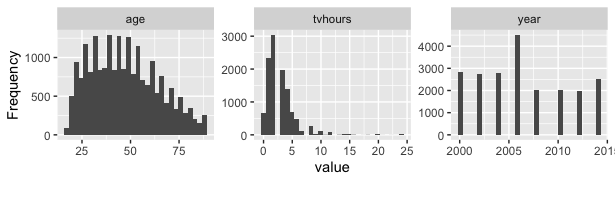
\includegraphics[width=7in]{01/fig-gss-histos.png}

We can compare side-by-side \textbf{\colorb{boxplots}} to look for relationships between two or more variables.

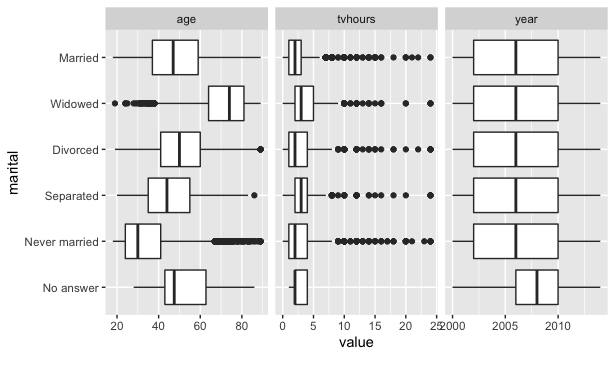
\includegraphics[width=7in]{01/fig-plot-boxplots.png}

\bbox
Married people tend to be older than people that have never been married, though there are a number of outliers.
\ebox

\clearpage

\pagebegin{Statistical Inference}

\bbox
\bi
\ii A \textbf{\colorb{population}} includes all individuals or objects of interest.
\ii A \textbf{\colorb{sample}} is a subset of the population.
\ii \textbf{\colorb{Statistical inference}} is the process of drawing conclusions about the entire population based on information in a sample.
\ii This semester we will \textbf{\colorr{focus on inference}}, and we will need some \textbf{\colorg{probability}} to do so.
\ei
\ebox

\begin{center}
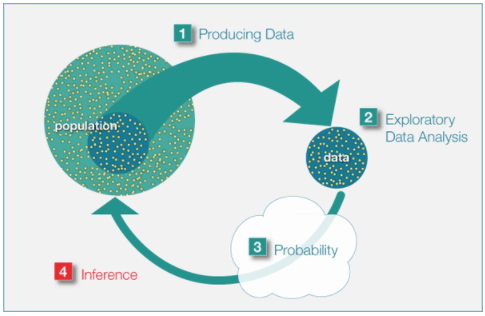
\includegraphics[width=6in]{01/fig-inference.png} %https://bolt.mph.ufl.edu/6050-6052/unit-4/
\end{center}

\bb[resume]
\ii In the GSS data example, is the data from a sample or a population? \vfill
\ii What statistical questions might be worth investigating among the 9 variables: year, marital, age, race, income, partyid, relig, denom, tvhours. \vfill
\ee

\clearpage

\pagebegin{Collecting Data: Sampling}


Since drawing a sample that resembles the population in every way (except smaller in number) is critical for drawing valid conclusions, how we pick samples is sometimes the most important step.


\begin{center}
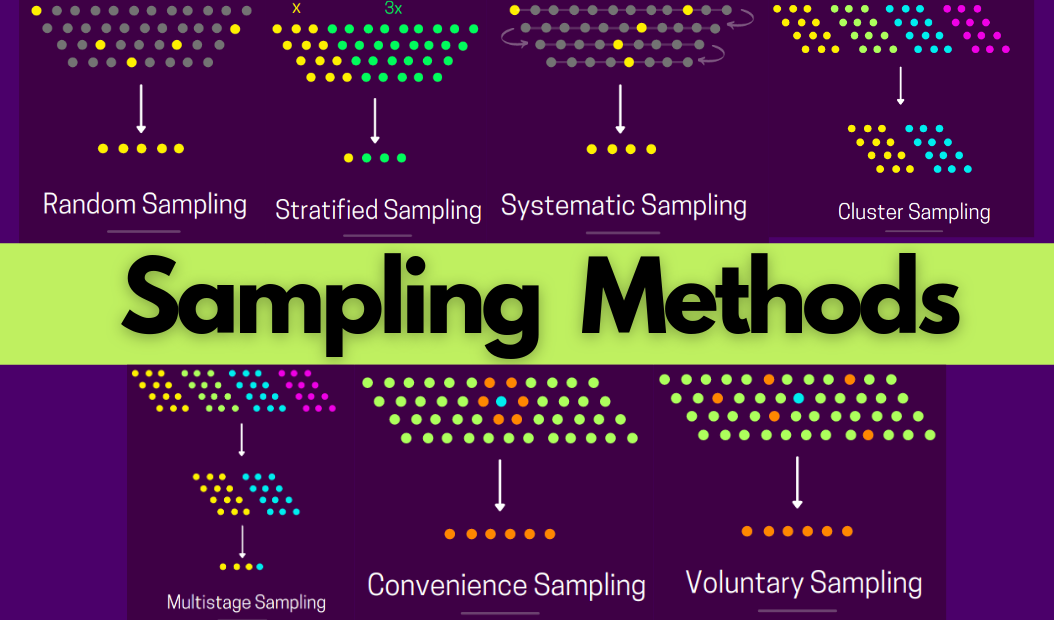
\includegraphics[width=6in]{01/fig-sampling-methods.png}
\end{center}
%https://towardsdatascience.com/8-types-of-sampling-techniques-b21adcdd2124 Prakhar Mishra

\bi
\ii When selecting a \colorb{simple random sample}, all individuals are equally likely to be selected.
\ii When selecting a \colorb{stratified sample}, the population is subdivided into groups based on some meaningful characteristic.
\ii When selecting a \colorb{systematic sample}, the first individual is chosen at random. Then a rule is used so that every $\mbox{n}^{\mbox{th}}$ individual is selected after that.
\ii When selecting a \colorb{cluster sample} groups rather than individual units of the target population are selected at random for the test. For example, only people with last digit of phone number equal to 8 are chosen.
\ii A \colorr{convenience sample} is when people or elements in a sample are selected on the basis of their accessibility and availability.
\ii \colorr{Voluntary sampling} is a type of a convenience sample;
\ei


\bbox
\textbf{\colorb{Sampling bias}} occurs when the method of selecting a sample causes the sample to differ from the population in some relevant way. Randomly selecting samples is the best way to avoid bias!
\ebox


\clearpage

\pagebegin{Collecting Data: Designing Studies}

Often in statistics we would like to investigate whether one variable is associated to another. Researchers carry out studies to understand the conditions and causes of certain outcomes.

\bi
\ii Does smoking cause lung cancer?
\ii Is paying people or punishing people a more effective incentive to get vaccinated?
\ii Is a new vaccine effective at preventing disease?
%\ii What factor is most significantly contributing to climate change?
\ei

\bbox
If we are using one variable to help us understand or predict the values (or category) of another variable, we call the first variable the \textbf{\colorb{explanatory variable}} and the second the \textbf{\colorb{response variable}}.
\ebox

\bb[resume]
\ii Both studies below are designed to examine determine whether rewarding good behavior or punishing bad behavior is a more effective method to help people quit smoking. Which study do you believe is better designed? Why?

\bb
\ii Employees at a large company voluntarily enroll in a quit smoking study. When they join, they are provided two options to select from:
\bi
\ii Option 1 (Reward-based group): If after six months the participant has quit smoking, they get an \$800 reward.
\ii Option 2: (Deposit-based group): Pay an initial \$150 refundable deposit. If after six months the participant has quit smoking, they receive their \$150 deposit back plus an additional \$800 reward. If they have not quit smoking, then they do not receive their \$150 deposit back.
\ei
After six months, the success rate is compared between the two groups.

\ii  Employees at a large company voluntarily enroll in a quit smoking study. When they join, they are randomly assigned to either be in the Reward-based or Deposit-based group (same as described above). After six months, the success rate is compared between the two groups.
\ee
\ee

\vfill

\begin{multicols}{2}

\bbox
A third variable that is associated with both the explanatory variable and the response variable is called a \textbf{\colorb{confounding variable}}.
\ebox

\columnbreak

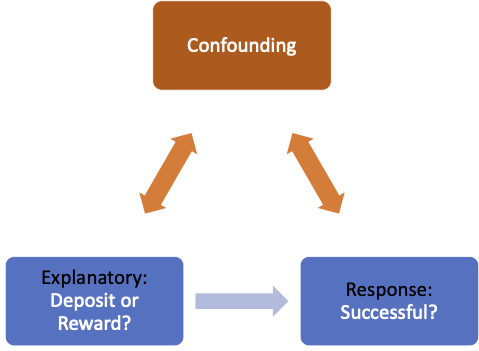
\includegraphics[width=0.45\tw]{01/fig-confounding.png}

\end{multicols}

\clearpage

\pagebegin{Experiments and Observational Studies}

\bbox
\bi
\ii An \textbf{\colorb{observational study}} is a study in which the researcher does not actively control the value of any variable.
\ii An \textbf{\colorb{experiment}} is a study in which the researcher actively controls one or more of the explanatory variables.
\ii The different categories of the explanatory variable are called \textbf{\colorb{treatments}}.
\ii In a \textbf{\colorb{randomized experiment}} the explanatory variable for each unit is determined randomly,
before the response variable is measured.
\ii If treatment groups are randomly determined, they should be similar in every way except for the treatment.
\ii \colorr{There are almost always confounding variables in observational studies.  Thus observational studies can almost never be used to establish causation.}
\ei
\ebox

\ms

% https://www.nsf.gov/pubs/2007/nsf0748/nsf0748_3.pdf

\textbf{An Overview of the General Social Survey}\ss

The General Social Survey (GSS) has provided a wealth of data on contemporary American society for approximately 35 years by measuring social change and trends and constants in attitudes, behaviors and attributes of the adult population. The GSS is a regular, ongoing interview survey of U.S households conducted by the National Opinion Research Center. The mission of the GSS is to make timely, high-quality, scientifically relevant data available to social science researchers. The GSS is a personal interview survey and collects information on a wide range of demographic characteristics of respondents and their parents; behavioral items such as group membership and voting; personal psychological evaluations, including measures of happiness, misanthropy, and life satisfaction; and attitudinal questions on such public issues as abortion, crime and punishment, race relations, gender roles, and spending priorities.

Since 1972 the GSS has conducted 26 in-person, cross-sectional surveys of the adult household population of the U.S. Interviews have been conducted with a total of 51,020 respondents. The 1972-74 surveys used modified probability designs and the remaining surveys were completed using a full-probability sample design, producing a high-quality, representative sample of the adult population of the U.S. The GSS has a response rate of over 70 percent above that of other major social science surveys and 40-45 percentage points higher than the industry average


\ms

 \textbf{Current GSS Design} \ss

The basic GSS design is a repeated cross-sectional survey of a nationally representative sample of non-institutionalized adults who speak either English or Spanish. Subsampling of non- respondents is done to limit survey costs while maintaining a nationally representative sample. Each GSS formally includes an A sample and a B sample. The preferred interview mode is in- person interviews; however, a few interviews will be done by telephone in the event that an in- person contact cannot be scheduled. Each respondent is asked the replicating core of socio- demographic background items, along with replicated measurements of sociopolitical attitudes and behaviors. Many of the latter are measured by way of a “ballot” design such that each item is answered by a random 2/3 of each sample. Each GSS sample (A and B) includes an International Social Survey Program module (ISSP). Each sample is also asked to respond to several topical modules that may be supported by NSF or others, but are no longer supported by the basic grant from NSF. Some of these topical modules, however, extend across both samples in a given GSS survey.

